\section{Experiments}

% ── Benchmark Dataset ─────────────────────────────────────────────────
\begin{frame}{Benchmark Dataset}
  \small
  \begin{columns}[T]
    \begin{column}{0.48\textwidth}
      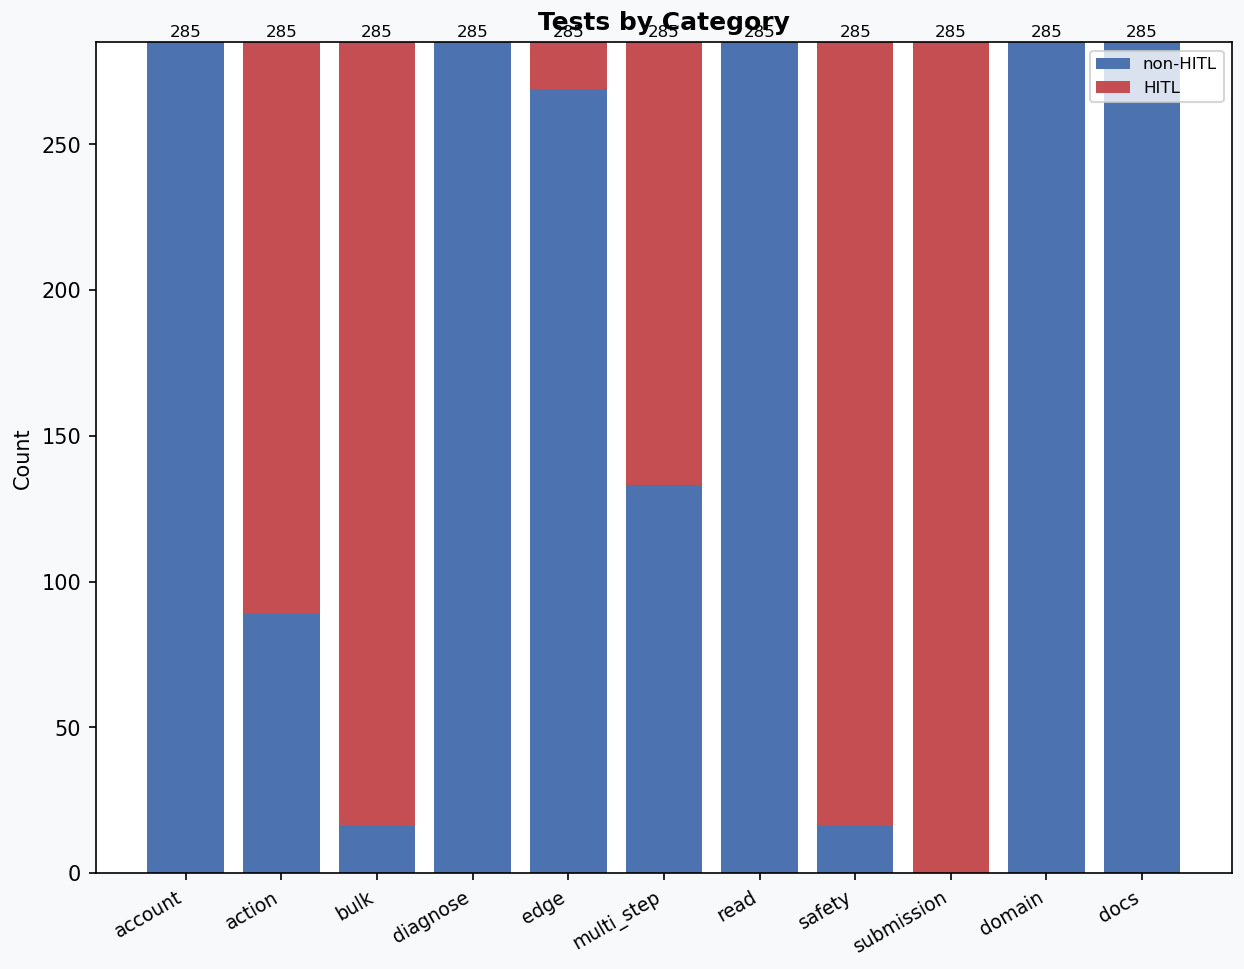
\includegraphics[width=\linewidth, height=5.5cm, keepaspectratio]{../report/images/evaluation/dataset_distribution_category.png}
      \captionof{figure}{11 categories, 285 cases each}
    \end{column}
    \begin{column}{0.48\textwidth}
      \begin{itemize}\setlength{\itemsep}{2pt}
        \item \textbf{11 categories}: read, diagnose, action, bulk, safety, submission, multi\_step, account, edge, docs, domain
        \item Each case: expected tools, routing label, HITL policy, keywords, source/target state
        \item 80/20 stratified split, seed=42
        \item \textbf{615-case held-out test set} for all model comparisons
        \item Mock Slurm state reset before each case
      \end{itemize}
    \end{column}
  \end{columns}
\end{frame}

% ── Evaluation Scoring ────────────────────────────────────────────────
\begin{frame}{Scoring Methodology}
  \textbf{3-way comparison (dual-agent):}
  \[
    \Large s = 0.35\,r_{\text{tool}} + \mathbf{0.25\,r_{\text{route}}} + 0.25\,r_{\text{HITL}} + 0.15\,r_{\text{state}}
  \]
  \vspace{-0.8em}
  \centering
  \renewcommand{\arraystretch}{1.1}
  \footnotesize
  \begin{tabular}{lrl}
    \toprule
    Dimension & Weight & Rationale \\
    \midrule
    Tool recall   & 35\% & Wrong tool $\Rightarrow$ wrong action \\
    Routing match & 25\% & Core safety claim \\
    HITL match    & 25\% & Core safety claim \\
    State match   & 15\% & Side-effect correctness \\
    \bottomrule
  \end{tabular}
  \flushleft
  \vspace{0.4em}
  \textbf{Ablation (dual vs.\ mono):} routing removed, weights $\times\,4/3$
  \[
    \Large s_{\text{abl}} = \frac{7}{15}\,r_{\text{tool}} + \frac{1}{3}\,r_{\text{HITL}} + \frac{1}{5}\,r_{\text{state}}
  \]
  \vspace{-0.8em}
  \footnotesize
  \flushleft
  Keyword excluded. Mean over $k{=}3$ trials, temperature~0.
\end{frame}

% ── Systems Evaluated ─────────────────────────────────────────────────
\begin{frame}{Testing Environment}
  \renewcommand{\arraystretch}{1.25}
  \begin{tabular}{llll}
    \toprule
    \textbf{System} & \textbf{Arch} & \textbf{Adapter} & \textbf{Role} \\
    \midrule
    GPT-5-mini            & Dual-agent & — (API)   & Commercial baseline \\
    \textbf{FT Qwen2.5-14B} & Dual-agent & QLoRA     & \textbf{Ours} \\
    Base Qwen2.5-14B      & Dual-agent & None      & Open-weight control \\
    Mono Qwen2.5-14B      & Monolithic & None      & Architecture ablation \\
    \bottomrule
  \end{tabular}
  \vspace{0.6em}

  \textbf{Protocol}
  \begin{itemize}\setlength{\itemsep}{3pt}
    \item 615-case held-out test set — identical for all models
    \item $k{=}3$ independent trials, temperature~0; mean score reported
    \item Mock Slurm state reset before each case
    \item LLM-as-judge: GPT-OSS 20B (Ollama, local), scores 0--1, reported separately
  \end{itemize}
\end{frame}
